Regeringen stiller en række krav til skolerne under skemaplanlægningsprocessen, der giver rammer skemaet bliver nødt til at holde sig indenfor. ''I Bekendtgørelsen af lov om folkeskole'' er tre fagblokke beskrevet. De humanistiske fag, praktiske/musiske fag og naturfaglige fag. Det er vigtigt, at løsningen kan overholde de lovmæssige krav, der stilles. En casestudy, som vil inddrages senere, vil bearbejde dette problem yderligere. Her opstilles kravene for de forskellige fag, som eleverne i den 9-årige grundskoleuddannelse skal følge.\footfullcite{lov2016} På figur~\ref{fig:Time} ses hvilke fag hvert klassetrin skal have undervisning i.

\begin{figure}[!hb]
  \centering
  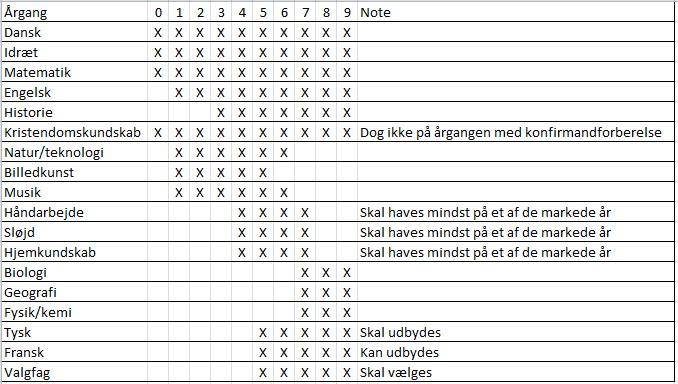
\includegraphics[width=\textwidth]{partials/graphics/fagkrav.png}
  \caption{Kravene for hvilke fag de enkelte årgange skal have.\footfullcite{lov2016}}
  \label{fig:Time}
\end{figure}

Valgfag består af følgende fag/emner: Tysk, fransk, spansk, medier, billedkunst, filmkundskab, drama, musik, håndarbejde og design, sløjd, madkundskab, motorlære, almindelige indvandrersprog for elever med tilstrækkelig kendskab til det sprog og arbejdskendskab. Valgfag skal være bestående af mindst 120 undervisningstimer årligt.\footfullcite{lov2016}
\\\\
En undervisningstime er, ifølge førnævnte bekendtgørelse, lig med 60 minutter. Børnehave og fra første til tredje klasse må ikke overskride undervisningstid over seks undervisningstimer om dagen, udover ved særlige arrangementer. Som ses på figur~\ref{fig:Timetal} er minimumskravet for første klasse 750 timer på et 200 dags skoleår, hvilket udgør 18,75 undervisningstimer ugentligt.\footfullcite{timeskema2016}

Medtages undervisningens vejledende timeantal er længden 30 timer ugentligt for en første klasse. For samtlige klasser betyder det følgende antal timer ugentligt:

•	Børnehave, første, anden og tredje klasse: 30 timer.

•	Fjerde, femte og sjette klasse: 33 undervisningstimer.

•	Syvende, ottende og niende klasse: 35 undervisningstimer.


\begin{figure}[!hb]
  \centering
  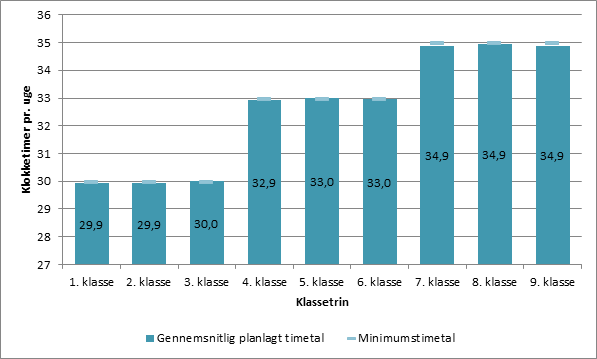
\includegraphics[width=\textwidth]{partials/graphics/planlagttime.png}
  \caption{Gennemsnitligt planlagttimetal kontra minimumstallet for 1.-9.-klasse.\footfullcite{timefolke2016}}
  \label{fig:ugetal}
\end{figure}

Dette stemmer overens med figur~\ref{fig:ugetal}.\footfullcite{timetalifolkeskolen2016} Dog skal det noteres at for alle fag ekskluderende, dansk matematik og historie \footfullcite{dennyefolkeskole} er disse vejledende timeantal. De skal  også opfylde undervisningstidens samlede længde, der ses nederst på figur~\ref{fig:Timetal}. Pauser indgår også i denne undervisningstid.\footfullcite{lov2016}

\begin{figure}[!ht]
  \centering
  \includegraphics[scale = 1]{partials/graphics/overallskemaovertimetal.png}
  \caption{Skema af kravene af timetal fra folkeskoleklasserne 0.- 9.\footfullcite{timeskema2016}}
  \label{fig:Timetal}
\end{figure}
 	
\subsubsection{Skolereformen}
I 2014 blev den nye skolereform introduceret i folkeskolerne. Reformen opstillede tre klare mål for folkeskolerne:\footfullcite{dennyefolkeskole}

•	Folkeskolen skal udfordre alle elever, så de bliver så dygtige, de kan.

•	Folkeskolen skal mindske betydningen af social baggrund for de faglige resultater.

•	Tilliden til og trivslen i folkeskolen skal styrkes blandt andet gennem respekt for professionel viden og praksis.

Målene bliver mødt ved længere skoledage, der giver de mindste elever en skoledag, som slutter omkring kl 14, fjerde til sjette klasse er det 14:30 og syvende til niende til 15. Den ekstra skoletid skal bl.a. støtte eleverne i bedre faglig fordybelse i særligt udfordrende fag ved brug af lektiehjælp. Udover dette bliver flere timer introduceret i form dansk og matematik fra fjerde til niende klasse. Engelsk, andet fremmedsprog og tredje fremmedsprog skal introduceres i henholdsvis første, femte og syvende klasse.\footfullcite{dennyefolkeskole}
Skolereformen har yderligere fokus på hævning af de pædagogiske kompetencer hos lærerne.
